% IMPORTANT
 
% Install tex distribution
% https://www.latex-project.org/get/
% With Windows, install MikTeX
 
% in RStudio, install.packages("knitR")
% also, install all packages that appear in first code chunk in this file, i.e. in the one that looks like this
% <<LoadingPackages, include=FALSE>>=
% library(knitr)
% library(xtable)
% library(dplyr)
% library(stargazer)
% library(cowplot)
% @

% Go to Tools/Global Options/Sweave
% Select Weave Rnw files using: knitr
% Select Typeset LaTeX into PDF using: pdfLaTeX
 
% Use button "Compile PDF" to knit the Rnw file to a tex file and compile the tex file to a pdf file.

% Always install all packages that you're asked to after having pressed "Compile PDF".
 
% If there is no error while knitting from Rnw to tex, but an error while compiling from tex to pdf, have a look at the pdf file. It might still have worked.



% Julian's suggestions from February 24

% Freitag: 
% - CD mit Daten, do-files
% - Codebook in Anhang 
% 
% soll nicht nach Evaluation durch LMU klingen
% 
% Seitenbegrenzung egal
% 
% Cronbach's alpha
% 
% immer robuste Standardfehler
% 
% i.year i.id
% 
% leading trailing - abdiskontieren
% 
% thematisch gegliederter Appendix






% Load graphicx package in your document's preamble
% Gandrud (2016), p.192

% turn page 90 degrees with lscape Gandrud (2016), p.185

% Create clickable hyperlinks with hyperref package, Gandrud (2016), p. 218

% Use natbib package for bibliography formatting, authoryear for Harvard style , Gandrud (2016), p. 227
% commands to change what information is included in the parentheses, Gandrud (2016), p. 228, table 11.2

% Using saveRDS and readRDS, following 
% https://csgillespie.github.io/efficientR/efficient-inputoutput.html#efficient-data-export-.rdata-or-.rds

% working with knitR and LaTeX
% https://kbroman.org/knitr_knutshell/pages/latex.html
% Command line
% R -e 'library(knitr);knit("knitr_example.Rnw")'

% rotate tables in knitr
% https://stackoverflow.com/questions/21840878/rotate-a-table-from-r-markdown-in-pdf
% in particular stargazer tables
% https://stackoverflow.com/questions/31169845/rotate-stargazer-table-in-knitr/34292292#34292292

% Create list of packages used, Gandrud (2016), p 218/219



% models with robust standard errors texreg
% https://github.com/DeclareDesign/estimatr/issues/316

\documentclass[12pt, a4paper, titlepage]{article}\usepackage[]{graphicx}\usepackage[]{color}
% maxwidth is the original width if it is less than linewidth
% otherwise use linewidth (to make sure the graphics do not exceed the margin)
\makeatletter
\def\maxwidth{ %
  \ifdim\Gin@nat@width>\linewidth
    \linewidth
  \else
    \Gin@nat@width
  \fi
}
\makeatother

\definecolor{fgcolor}{rgb}{0.345, 0.345, 0.345}
\newcommand{\hlnum}[1]{\textcolor[rgb]{0.686,0.059,0.569}{#1}}%
\newcommand{\hlstr}[1]{\textcolor[rgb]{0.192,0.494,0.8}{#1}}%
\newcommand{\hlcom}[1]{\textcolor[rgb]{0.678,0.584,0.686}{\textit{#1}}}%
\newcommand{\hlopt}[1]{\textcolor[rgb]{0,0,0}{#1}}%
\newcommand{\hlstd}[1]{\textcolor[rgb]{0.345,0.345,0.345}{#1}}%
\newcommand{\hlkwa}[1]{\textcolor[rgb]{0.161,0.373,0.58}{\textbf{#1}}}%
\newcommand{\hlkwb}[1]{\textcolor[rgb]{0.69,0.353,0.396}{#1}}%
\newcommand{\hlkwc}[1]{\textcolor[rgb]{0.333,0.667,0.333}{#1}}%
\newcommand{\hlkwd}[1]{\textcolor[rgb]{0.737,0.353,0.396}{\textbf{#1}}}%
\let\hlipl\hlkwb

\usepackage{framed}
\makeatletter
\newenvironment{kframe}{%
 \def\at@end@of@kframe{}%
 \ifinner\ifhmode%
  \def\at@end@of@kframe{\end{minipage}}%
  \begin{minipage}{\columnwidth}%
 \fi\fi%
 \def\FrameCommand##1{\hskip\@totalleftmargin \hskip-\fboxsep
 \colorbox{shadecolor}{##1}\hskip-\fboxsep
     % There is no \\@totalrightmargin, so:
     \hskip-\linewidth \hskip-\@totalleftmargin \hskip\columnwidth}%
 \MakeFramed {\advance\hsize-\width
   \@totalleftmargin\z@ \linewidth\hsize
   \@setminipage}}%
 {\par\unskip\endMakeFramed%
 \at@end@of@kframe}
\makeatother

\definecolor{shadecolor}{rgb}{.97, .97, .97}
\definecolor{messagecolor}{rgb}{0, 0, 0}
\definecolor{warningcolor}{rgb}{1, 0, 1}
\definecolor{errorcolor}{rgb}{1, 0, 0}
\newenvironment{knitrout}{}{} % an empty environment to be redefined in TeX

\usepackage{alltt}
\usepackage{lscape}
\usepackage{graphicx}
\usepackage[utf8]{inputenc}
\usepackage[backend=biber, bibstyle=apa, citestyle=authoryear]{biblatex}
\usepackage{floatrow}
\usepackage{booktabs}
\usepackage[hidelinks]{hyperref}
\usepackage{rotating}
% \usepackage[authoryear]{natbib}
% \bibliographystyle{apalike}
\usepackage{mathtools}
\usepackage[onehalfspacing]{setspace}
\usepackage[left = 2.5cm, top = 2.5cm, right = 2.5cm, bottom = 2.0cm]{geometry}

% 1.5 spacing in Word is about this in LaTeX
% https://tex.stackexchange.com/questions/65849/confusion-onehalfspacing-vs-spacing-vs-word-vs-the-world

\linespread{1.25}

\addbibresource{references.bib}






% multiple authors
% https://tex.stackexchange.com/questions/4805/whats-the-correct-use-of-author-when-multiple-authors

\title{Effects of CHILDREN's programs}
\author{
Laura Huber\\
\texttt{11111111}
\and
Laura Jepsen\\
\texttt{11567799}
\and
Jonathan Kirschner\\
\texttt{11724530}
\and
Rafael Schütz\\
\texttt{11574909} 
\and 
Yannick Zurl\\
\texttt{11111111}
\and
Studentisches Praxisprojekt zur Empirischen Wirtschaftsforschung PaRE3To\\
\and
Ludwig-Maximilians-Universität Munich
}


% Winter Term 2019/20\\

\date{27th February 2020}
\IfFileExists{upquote.sty}{\usepackage{upquote}}{}
\begin{document}

% \begin{titlepage}
\maketitle
% \end{titlepage}

\tableofcontents
\listoftables

% note below table
% https://stackoverflow.com/questions/44549464/table-spacing-issue-converting-to-pdf-via-latex-with-pandoc/44797387#44797387
\listoffigures

\begin{abstract} 
abstract on separate page
100 - 150 words
\end{abstract}

\section{Formal requirements}
all important information on title page, maybe use template\\
always name sources of tables and graphs\\
have to cite data sets\\
latin number pages\\


\section{Examples}

Equation with double index\\

\begin{equation}
\label{ModelProdu}
\ln y_{it}^{n} = \beta_0 + \beta_k \ln k_{it-1}^{n} + \beta_n \ln n_{it} + \beta_m \ln m_{it} + \beta_t D_t + \beta_i D_i + \epsilon_{it}
\end{equation}

List\\

\begin{itemize}
  \item{The firm is not incorporated in the U.S. (FIC is not equal to USA.)}
  \item{The company is from the financial or utilities sector. This is the case when the SIC code lies between 4900 and 4999 or between 6000 and 6999.}
  \item{A firm's acquisitions are larger than five percent of the value of its total assets. This is the case when AQC over AT is larger than 0.05.} 
\end{itemize}


Figure\\

\begin{figure}
  \caption{Dispersion in productivity levels}
  \label{LineDisp}

\begin{knitrout}
\definecolor{shadecolor}{rgb}{0.969, 0.969, 0.969}\color{fgcolor}

{\centering 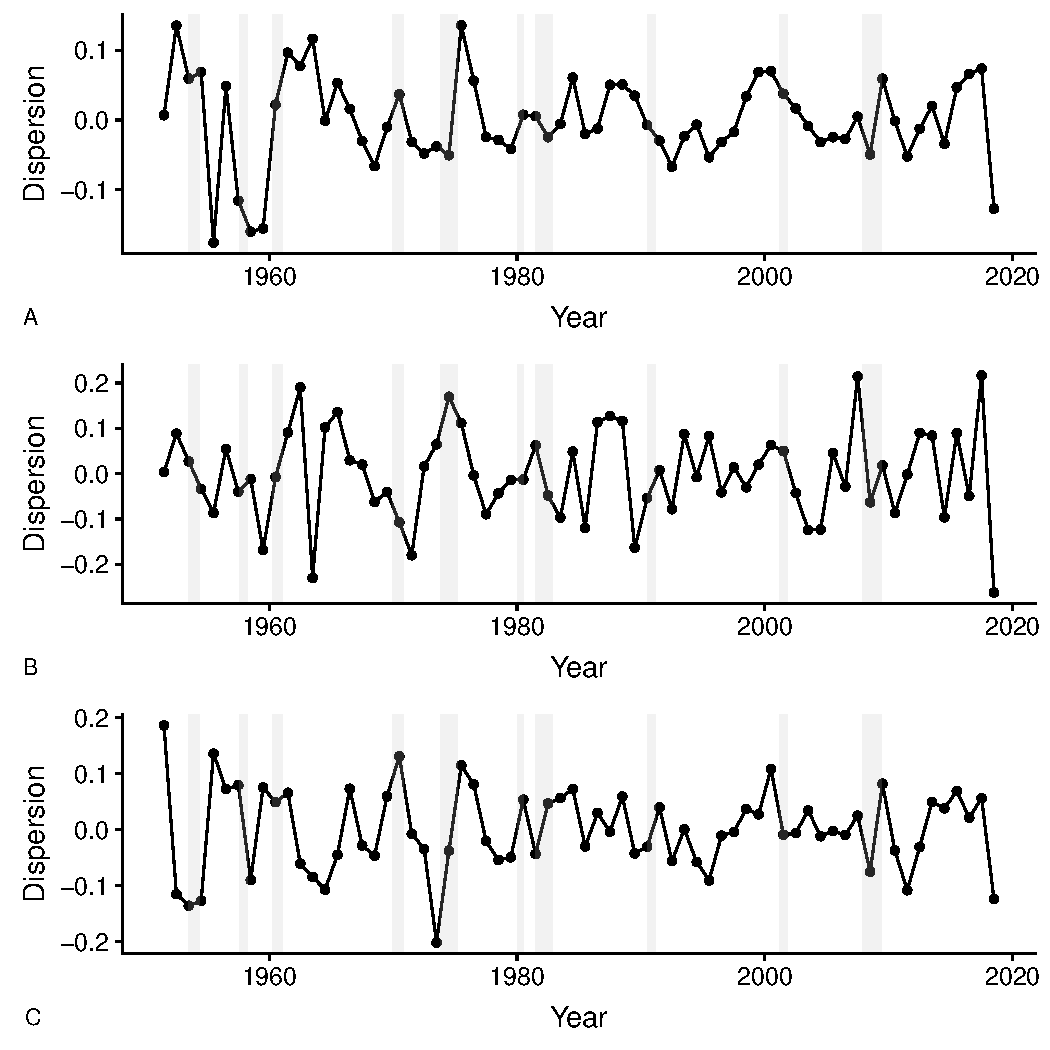
\includegraphics[width=0.8\textwidth]{figure/unnamed-chunk-1-1} 

}



\end{knitrout}

\floatfoot{Note: Time series plots of approximate deviations of the three annual dispersion measures from their trends in percent. A shows the full sample, B the non-durable manufacturing sector, and C the durable manufacturing sector. After taking the natural logarithm of the dispersion measures defined in equation 1, I have isolated their cyclical components with an HP-100 filter. The shaded bars represent recessions as defined by the NBER. The year ticks refer to January 1. The dispersion measures take as their date the middle of the year, July 2. Compare Kehrig (2015), Figure 1.}
\end{figure}


Figure \ref{LineDisp}

% <<results='asis', echo=FALSE>>=
% tableCyclicDisp = readRDS("./Analysis/CyclicDisp.Rds")
% colnames(tableCyclicDisp) <- c("Lead in years", "All", "p-value", "Non-Durables", "p-value", "Durables", "p-value")
% tableCyclicDisp <- xtable(tableCyclicDisp, caption = "Cyclicality of productivity dispersion", digits = c(0, 0, 3, 2, 3, 2, 3, 2))
% print(tableCyclicDisp, include.rownames = FALSE)
% @

Regression fit output with texreg\\


\begin{table}
\begin{center}
\begin{tabular}{l c c }
\hline
 & Model 1 & Model 2 \\
\hline
(Intercept)      & $-12089.14^{*}$ & $3.70^{***}$ \\
                 & $(5192.86)$     & $(0.33)$     \\
realSubsidy      & $2.61^{***}$    &              \\
                 & $(0.57)$        &              \\
realTripsSubsidy &                 & $0.00^{*}$   \\
                 &                 & $(0.00)$     \\
\hline
R$^2$            & 0.43            & 0.05         \\
Adj. R$^2$       & 0.43            & 0.04         \\
Num. obs.        & 329             & 322          \\
RMSE             & 39992.79        & 2.96         \\
\hline
\multicolumn{3}{l}{\scriptsize{$^{***}p<0.001$, $^{**}p<0.01$, $^*p<0.05$}}
\end{tabular}
\caption{Statistical models}
\label{table:coefficients}
\end{center}
\end{table}


Table \ref{mealsTripsSubsidyRegressions}
% To have an unnumbered section, place an sterisk in it like this \*{Unnumbered Section}
\section{Outline}
Descriptive statistics\\
dynamics of\\ 
(- number of organizations)\\
(- number of beneficiaries)\\
- selected ordinal outcomes, stacked\\
- real total subsidy\\
- real median subsidy per institution\\
- real median subsidy per beneficiary\\
(- which variables have largest variance; also relevant for variable selection)\\

Regressions\\

Questions:\\
effect of\\
- healthy meals (DGE criterion) standardized on healthy characteristics standardized, with eatersPerMeal as weights\\
- real meals subsidy on number of meals\\
- real trips subsidy on number of trips\\
- real meals subsidy per beneficiary on standardized self-worth and standardized day-to-day skills\\
- real trips subsidy per beneficiary on standardized self-worth and standardized day-to-day skills\\

Methods:\\
- simple, metric\\
- standardized, metric\\
- cumulative logit\\
- with control variables\\
(- without outliers)\\
(- imputed data)\\

Diff in Diff\\

Outlook for CHILDREN/variable selection\\
- double selection \\
- partition analysis\\
(- correlation matrix)\\
(- factor analysis)\\
- general tips\\

\section{Introduction}

the introduction should include: motivation, precise research questions, very short literature review, most important results, further proceedings

CHILDREN's aims for data analysis\\ 
CHILDREN supports organizations working with children and youth across Germany (in German: Einrichtungen der offenen Kinder- und Jugendarbeit) across Germany. We call them organizations in the following. They apply to CHILDREN for yearly grants. If approved, they are supposed to use them for specific purposes defined by CHILDREN. CHILDREN provided us with data from two of its flagship programs: Mittagstisch (we refer to this as Meals program) and Entdeckerfonds (Trips program). The organizations use money from the Meals program to finance meals, from breakfast to dinner, that they sell at concessionary prices to the children and youth that visit them. In the following, we call these children and youth who ultimately profit from CHILDREN's grants beneficiaries. The organizations also use money from the Trips program to make trips to nearby places usually unknown to the beneficiaries.  
Unless otherwise specified, we consider all variables to be metric, even if they are ordinal. 

\section{Data}

To measure the effect of CHILDREN´s engagement on the organizations we use the data they collected from 2011 to 2018. In each year they send a survey to the organizations with several questions about the previous year. The number of organizations varies among the years and increases over time, from 52 in the 2012 survey to 73 in the survey from 2020. In some organizations one employee fills in the survey and in others they do it as a team. Since the children and adolescents are not questioned directly, all responses are documented through the perception of the employees. The number of variables varies over time as well. Included are numbers like the average eaters per meal or the amount of money they provide to the organizations but also general questions. For instance, CHILDREN asks the average amount of kids with a better confidence or an improved dietary knowledge in the specific organization. This part of the survey must be answered on a scale from zero (no kids) to four (all kids). If an organization do not answer a question, this is documented as a “99”. We worked with the statistical program “R” and therefore changed the format from 99s to NA´s (not available) to avoid distortions. The surveyed variables change over the years, but some of them are included every year. 
However, we did several steps to get a full dataset we could work with. The data was divided into one dataset for each survey from 2011 to 2019, but we only use the surveys till 2018 since in 2019 some organization-ID´s occurred several times and the data for 2019 were incomplete. Since each survey includes data about the year before, we changed the names of the dataset to the corresponding year and finally used the years from 2011 to 2018. Moreover, we outlined a hierarchical file structure, enabling us to use relative file paths throughout. This makes a quick work with R possible since we only use paths relative to the working directory. Afterwards we made sure that variables with names containing non-standard characters like German “Umlaute” are correctly read in and established naming conventions. We created a file reading the excel sheets and we reviewed and aligned new English-language variable names across the years. Moreover, we systematically compared variable names between years by creating a correspondence table, ordered first by variables of 2019, then of 2018 and so on. To ensure the comparability between the years, we gave all variables from the different years that equal each other the same name. As a next step, we merged the different datasets to one dataset, including all years and variables CHILDREN collected. For an efficient and clear data structure, we created a function that automatically changed the data type of all variables from "character" to "ordinal" and added several versions for each initially metric encoded variable afterwards. The three variants are ordinal, standardized and weighted (FUßNOTE: The variables regarding the Mittagstisch are weighted as variable*0.25*eaterspermeal, the variables that are assigned to the Entdeckerfonds as variable*0.25*tripskidsno). 
Furthermore, we created more new variables: We used the information CHILDREN gave us in another excel-sheet to assign the German states to the corresponding organization-ID and created dummy-variables for each ID, every year and a treatment dummy that will be explained in a later section. 
The final dataset we worked with is structured as follows: Each row represents one organization-ID with the answers the organization gave in the specific year. The questions are divided in two categories: the variables regarding to the Mittagstisch, answered by all organizations since they are all part of this program and the Entdeckerfonds variables, answered by the organizations that take part on the Entdeckerfonds program in the respective year. Including the years from 2011 to 2018 and all variables we created, the final dataset has X observations of Y variables.

Many organizations do not answer all questions CHILDREN poses. We create a seperate data set, in which we impute missing values with an organization-specific linear trend. CHILDREN supports some very large organizations that give out hundreds of meals a day or conduct dozens of trips per year. We fit our models with outliers excluded to see if they are driving results. We define an outlier as a value that is at least 1.5 interquartile ranges below the 25th percentile or equally far above the 75th percentile. Once we exclude outliers in terms of numbers of meals and once in terms of number of trips.

Figure\\

\begin{figure}
  \caption{Trend in everyday expertise and selfworth}
  \label{LineDisp}

\begin{knitrout}
\definecolor{shadecolor}{rgb}{0.969, 0.969, 0.969}\color{fgcolor}

{\centering 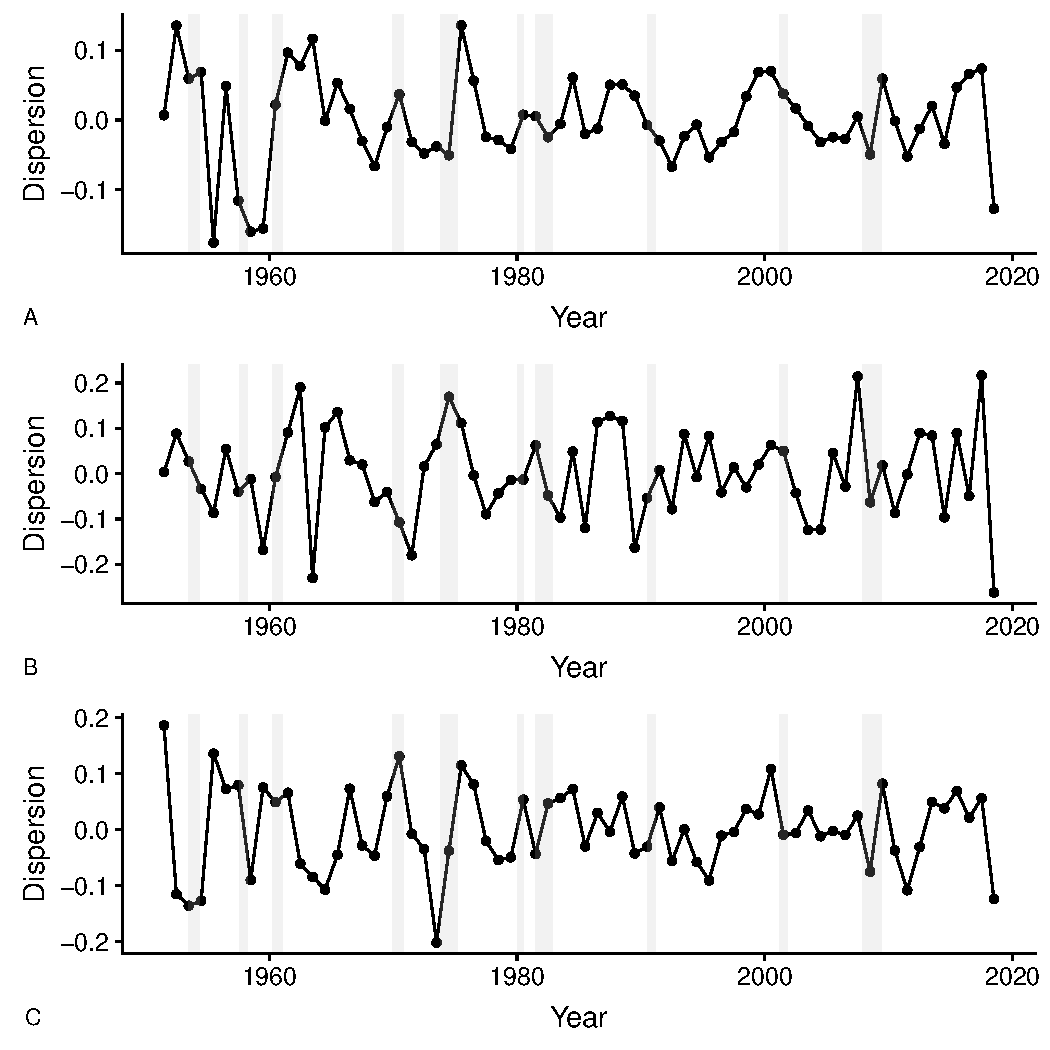
\includegraphics[width=0.8\textwidth]{figure/unnamed-chunk-2-1} 

}



\end{knitrout}

\floatfoot{Note: The x-axis represents the years from 2012 to 2018, the year 2011 is left out because the trips program starts in 2012. The y-axis represents the average answers from the organizations regarding to selfworth (graph x) and everyday expertise (graph y). The time trend of the average answers from the organizations in the treatment group is characterised by the solid line, the answers from the control group by the dotted line. Additionally, the linear trends of both groups are included as the straight lines.}
\end{figure}

\section{Summary Statistics}
\subsection{Fundamental Dynamics} 

In this section, we give an overview of the dynamics of CHILDREN's two flagship programs. We focus on the number of estimated ultimate beneficiaries in both programs, median total subsidy, median subsidy per institution, and median subsidy per beneficiary. We also look at selected outcomes, i.e. those related to health as well as self-worth and day-to-day skills. We have converted all nominal monetary variables into 2015 euros, using price indices from the Federal Statistical Office of Germany (Statistisches Bundesamt). We deflate (requested) grants as well as organizations' total expenses for the Meals program  with the price index related to food and non-alcoholic beverages (in German: Nahrungsmittel und alkoholfreie Getränke) and (requested) grants towards the Trips program with the price index for leisure, entertainment, and culture (in German: Freizeit, Unterhaltung und Kultur). These are only available after logging in on DESTATIS. The organizations also gave information about their total yearly budget. We inflate this with the general price index.

% latex table generated in R 3.6.2 by xtable 1.8-4 package
<<<<<<< HEAD
% Wed Feb 26 23:16:47 2020
=======
% Wed Feb 26 22:15:10 2020
>>>>>>> 72c6d5913679c3fb04935b691d8cdf7883ee60c8
\begin{table}[ht]
\centering
\begin{tabular}{mmmmm}
  \hline
Year & Beneficiaries, Meals & Beneficiaries, Trips & Organizations, Meals & Organizations, Trips \\ 
  \hline
2011 & 3748.0 &  & 52 &  \\ 
  2012 & 3556.0 & 2803.0 & 51 & 44 \\ 
  2013 & 4015.0 & 2823.0 & 55 & 42 \\ 
  2014 & 4685.0 & 2752.0 & 55 & 43 \\ 
  2015 & 5857.0 & 3823.0 & 55 & 49 \\ 
  2016 & 3075.0 & 3819.0 & 59 & 48 \\ 
  2017 & 4895.0 & 4150.0 & 64 & 48 \\ 
  2018 & 5102.5 & 6911.0 & 68 & 49 \\ 
   \hline
\end{tabular}
\caption{Summary Statistics} 
\label{fundamentalDynamics}
\end{table}

% look up official names of price indices in English 


Table \ref{fundamentalDynamics} shows that, at the beginning of the time series in 2011, in the Lunch program they supported in 52 organizations. In 2018, this number has increased to 68. In 2011, CHILDREN financed meals for 3748 beneficiaries, and for 5103 in 2018. In the trips program, which launched in 2012, the number of supported organizations amounted to 44 in 2012 and grew to 49 until 2018. In 2012, their grant allowed 2803 beneficiaries to go on trips, and 6911 in 2018.

\subsection{Trend of grants} 

\begin{figure}
  \caption{Yearly dynamics of total grants in Meals and Trips program}
  \label{totalGrantsDyn}

\begin{knitrout}
\definecolor{shadecolor}{rgb}{0.969, 0.969, 0.969}\color{fgcolor}

{\centering 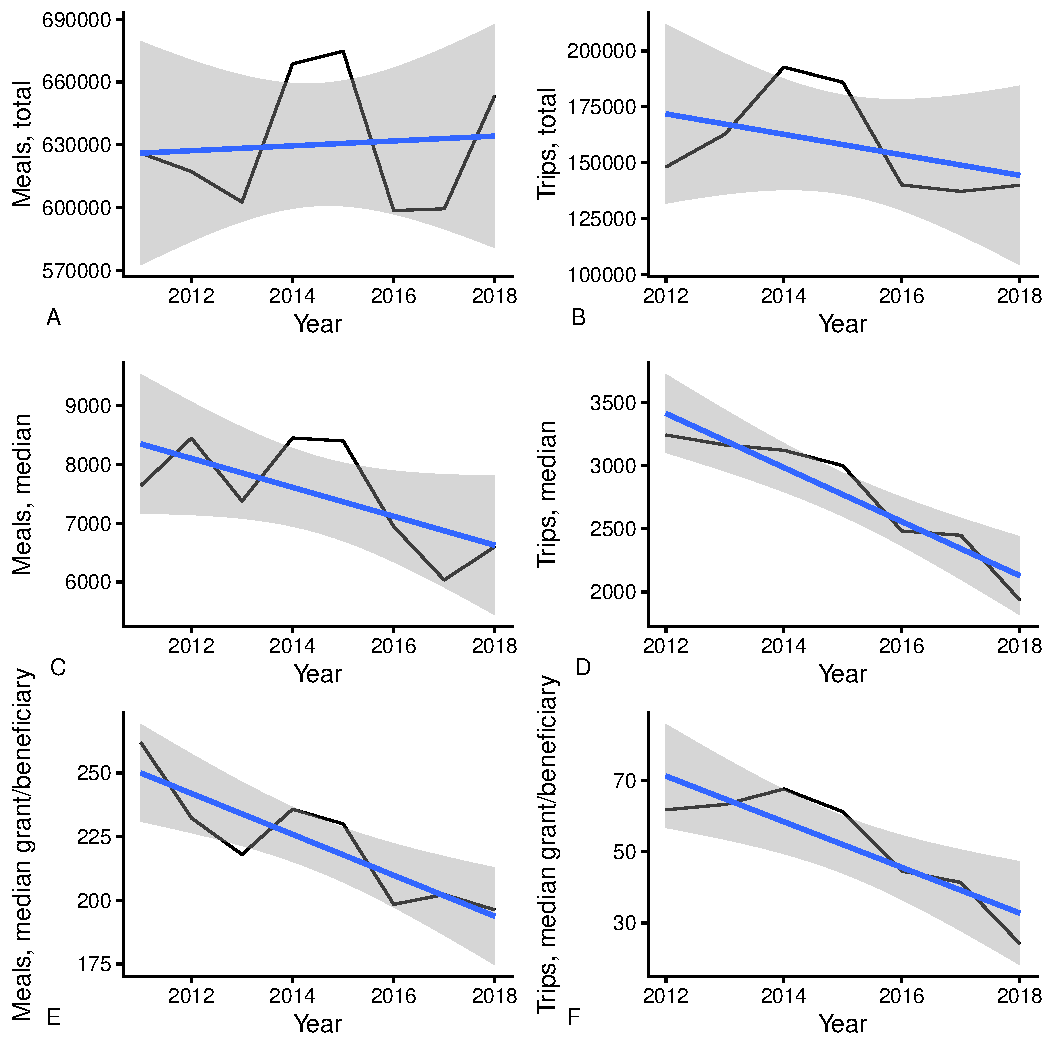
\includegraphics[width=0.8\textwidth]{figure/GrantTrend-1} 

}



\end{knitrout}

\floatfoot{This graph shows the development of grants in the Meals compared to the Trips program. We distinguish between the sum of grants in one year, the median grant and the median grant per beneficiary. From left to right: Meals, Trips. From top to bottom: sum, median, median per beneficiary. We have deflated the values to 2015 euros using the price index related to food and non-alcoholic beverages(in German: Nahrungsmittel und alkoholfreie Getränke) for the Meals program and the price index related to Leisure, Entertainment and Culture (in German: Freizeit, Unterhaltung, Kultur) provided by the Federal Statistical Office of Germany (Statistisches Bundesamt).}
\end{figure}

For the dynamics of figure \ref{totalGrantsDyn} we visualze the dynamics of CHILDRENs' grants by distinguishing between the sum of grants in one year, the median and the median grant per beneficiary. We also compare the grants of the Lunch and the Trips Program.

Figure \ref{totalGrantsDyn} shows no exact trend for the total real grant for the Lunch program. Between 2013 and 2015 the grant increased from about 600000 EUR to 680000 EUR, but falls behind in the following year. Since 2017 an increase is again visible. In comparison to this, there is a clearer negative trend in median Meals subsidy, falling from about 8000 EUR in 2012 to about 6500 EUR in 2018. In accordance, the median Meals grant per beneficiary shrinks from about 250 EUR to about 200 EUR. 

In the total Trips grant, a slightly negative trend is visible, after the subsidy increased to approximately 200000 EUR in 2014, but decreased to about 130000 EUR in 2016, and is connstand eversince. The Trips median grant therefore also decreased from 3000 EUR to 2000 EUR over the time period, as well as the median grant per beneficiary decreased from about 60 EUR to about 30 EUR.

These results visualize, for the Lunch as well as for the Trips program, together with the fundamental dynamics of table \ref{fundamentalDynamics}, that children was able to increase the number of organizations they support, but had to distribute the available subsidy among them. 

\subsection{Health relevant variables over time} 

In its yearly surveys, CHILDREN asks about three variables closley related to a healthy diet. These are the shares of beneficiaries who are healthier, have a growing appreciation for a healthy diet, or have increased their knowledge about what constitutes a healthy diet. Figure \ref{Health_timeplots} displays the share of organizarions in each category of the health outcome from 2011 to 2018. The possible values are: all(coded as 4), most (3), some (2), few (1), and none (coded as 0). For this figure, we use the original ordinal varibles which result from the survey structure.  

\begin{figure}
  \caption{Health outcome over time}
  \label{Health_timeplots}
\begin{knitrout}
\definecolor{shadecolor}{rgb}{0.969, 0.969, 0.969}\color{fgcolor}

{\centering 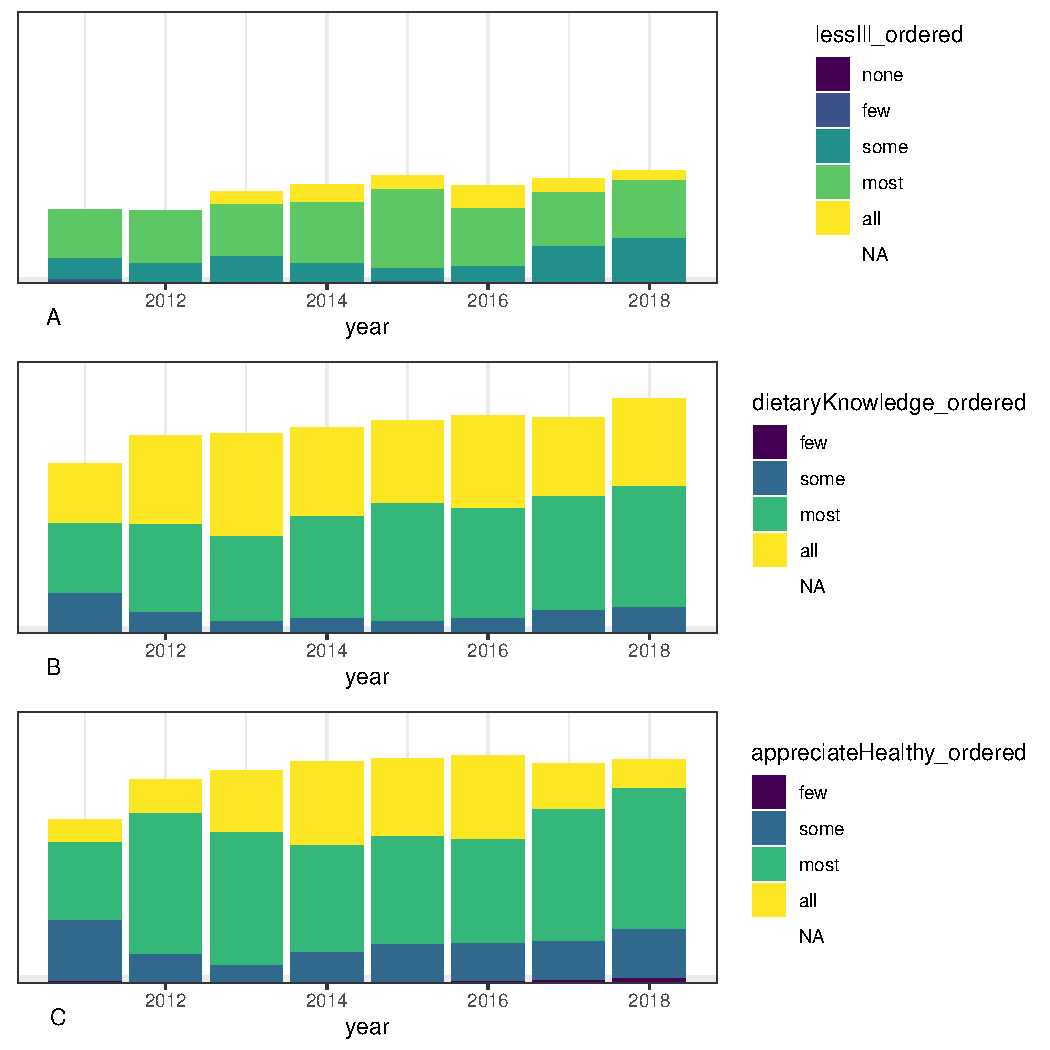
\includegraphics[width=0.8\textwidth]{figure/HealthTimePlots-1} 

}



\end{knitrout}
\floatfoot{In its yearly surveys CHILDREN asks about three variables closley related to a healthy diet. These are the shares of beneficiaries who are healthier (lessIll\_ordered), have a growing appreciation for a healthy diet (dietaryKnowledge\_ordered), or have increased their knowledge about what constitutes a healthy diet (appreciateHealthy\_ordered).
The x-axis plots the year. The y-axis displays the share of organizarions in each category of the health outcome. The possible values are: all(coded as 4), most (3), some (2), few (1), and none (coded as 0). For example, if an organization says that most beneficiaries are healthier, then this would be coded as 3.}
\end{figure}

In Figure \ref{Health_timeplots}, for the variable 'lessIll', there is much non available data. In all years, most organizations say that most beneficiaries are more healthy (3). The least stated category is, that all beneficiaries are less ill(4). That few are less ill (1), appears sometimes and the leftover category,none (0), which is only coded for the variable 'lessIll', appears as good as never.

In the second plot of figure \ref{Health_timeplots} (variable 'dietaryKnowledge') mostorganizations state, that predominantely most or all beneficiaries increased their knowledge about what constitutes a healthy diet. The least stated category is that some beneficiaries increased their dietary knowledge (2). The leftover category, few (1), does not appear.

The the bottom plot of figure \ref{Health_timeplots}, which visualizes the variable 'appreciateHealthy'. Again most organizations state, that most beneficiaries have a growing appreciation for a healthier diet (3). The second most stated answer is that all beneficiaries have a growing appreciation for a healthier diet (4). The least stated category by the organizations is, as well as in the second plot, that some have a growing appreciation for a healthier diet (2). The leftover category, few, also does not appear.


\subsection{Equality of opportunities releveant variables over time} 

In its yearly surveys, CHILDREN has always asked about two variables closley related to increasing the beneficiaries' equality of opportunities. These are the degree to which beneficiaries: have more selfworth and have a growing understanding for everyday expertise. Figure 4 displays the share of organizarions in each category of the health outcome from 2011 to 2018. The possible values are: all(coded as 4), most (3), some (2), few (1), and none (coded as 0). As well as in the last figure (figure 3), we use the original ordinal varibles which result from the survey structure.

\begin{figure}
  \caption{Equality of opportunities over time}
  \label{Equality_timeplots}
\begin{knitrout}
\definecolor{shadecolor}{rgb}{0.969, 0.969, 0.969}\color{fgcolor}

{\centering 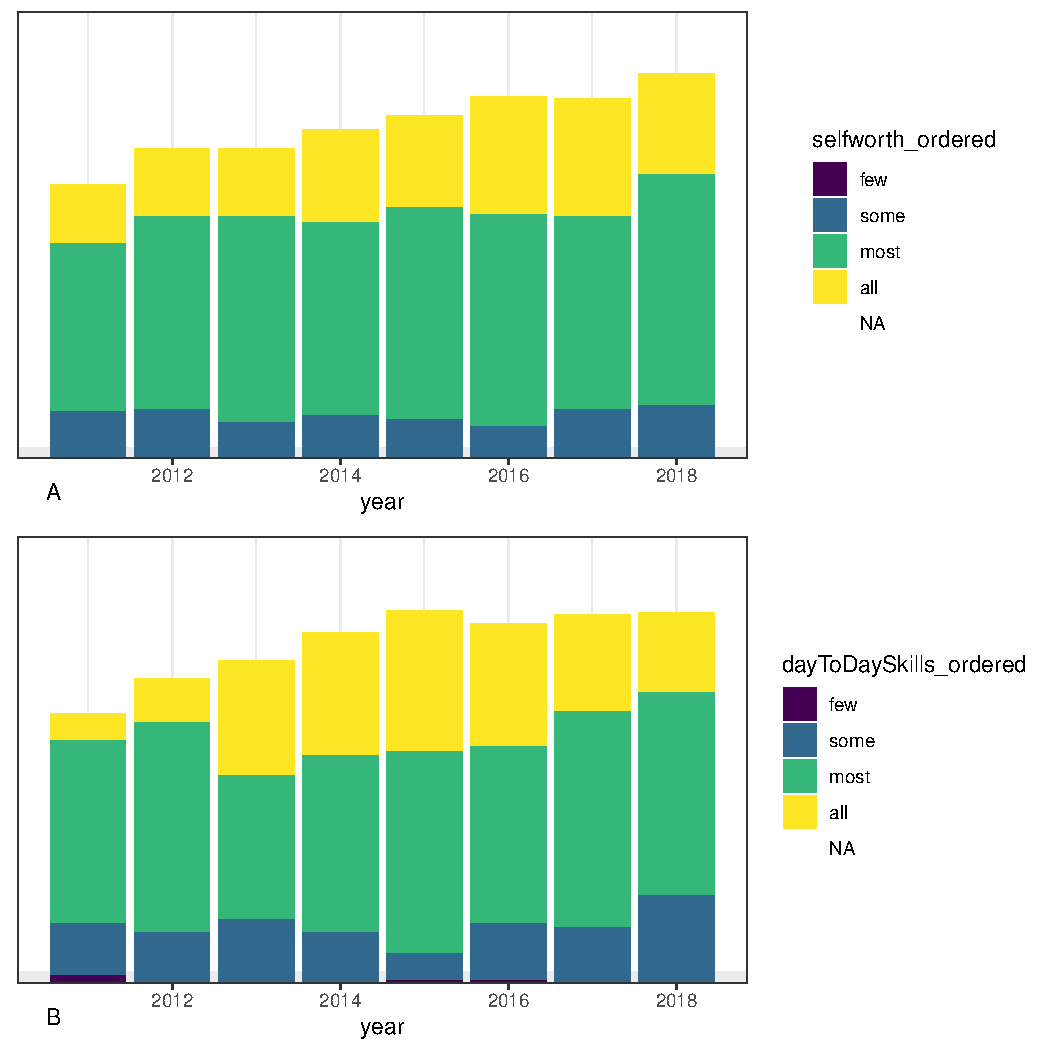
\includegraphics[width=0.8\textwidth]{figure/EqualityTimePlots-1} 

}



\end{knitrout}
\floatfoot{In its yearly surveys CHILDREN has always asked about two variables closley related to increasing the beneficiaries' equality of opportunities. These are the degree to which beneficiaries: have more selfworth (selfworth\_ordered) and have a growing understanding for everyday expertise (dayToDaySkills\_ordered).  
The x-axis plots the year. The y-axis displays the share of organizarions in each category of the health outcome. The possible values are: all(coded as 4), most (3), some (2), few (1), and none (coded as 0). For example, if an organization says that most beneficiaries have more selfowrth, then this would be coded as 3.}
\end{figure}

Figure 4 shows in its upper plot the development of the answered categories for the variable selfworth. Mostly, the answer is that most beneficiaries in most organizations have more selfworth (3). The second most stated category is that all beneficiaries gained in selfworth (4) and the least stated is that some have more selfworth (2). The leftover category, few, does not appear.

In the bottom plot of figure 4 the development of everyday expertise of the beneficiaries over time is visible. The results are about similar to the previous results of selfworth: Most beneficiaries in most organisations have a growing understanding for everyday expertise (3). 

\section{Regressions}

\subsection{Empirical Approach} 

\begin{equation}
\label{SimpleLinearModel}
  y_{it} = \beta_0 + \beta_1 x_{it} + \epsilon_{it}
\end{equation}


In this section we use a simple linear model, as described in equation \ref{SimpleLinear Model}. We look at the association between: 

\begin{itemize}
  \item{the subsidy (in 2015 EUR) an organization receives through CHILDREN's Meals program and the number of meals it dispenses}
  \item{the subsidy (in 2015 EUR) an organization receives through CHILDREN's Trips program and the number of trips it conducts}
  \item{the subsidy per beneficiary (in 2015 EUR) an organization receives through CHILDREN's Meals program and the standardized measure of beneficiaries' self-worth}
  \item{the subsidy per beneficiary (in 2015 EUR) an organization receives through CHILDREN's Meals program and the standardized measure of beneficiaries' everyday expertise}
   \item{a standardized measure of the healthiness of the meals an organization dispenses and various standardized health-related outcomes of beneficiaries} 
\end{itemize}

We discuss all these models in turn.

\subsection{Direct effects of CHILDREN's grants} 

If CHILDREN's grants are to have an effect on beneficiaries, they should first influence the output of organizations in terms of meals dispensed and trips conducted. 

As table \ref{GrantsRegressionsLunch} shows, this is emphatically true. Whether we look at the original data set, the one without outliers and the one with imputed values, a strong association becomes evident. 
The estimated coefficients are very similar when we use the original dataset and the one with imputed values. In the case of the original data set, increasing the subsidy to an organization by one EUR is associated with 2.6 additional meals dispensed. This estimate is highly statistically significant. When we exclude outliers, i.e. those organizations that give out very many menus or very few menus,
the estimated coefficient decreases by about one order of magnitude. Still, spending not much more than three EUR more goes hand in hand with one extra meal. The estimate is also highly statistically significant.  


\usepackage{booktabs}

\begin{table}
\caption{Regression Results: Number of meals}
\begin{center}
\scalebox{0.8}{
\begin{tabular}{l c c c }
\toprule
 & OLS & OLS without Outliers & OLS Impute \\
\midrule
(Intercept) & $-12089.14^{*}$ & $3535.39^{***}$ & $-12250.60^{**}$ \\
            & $(5192.86)$     & $(498.99)$      & $(4524.09)$      \\
realSubsidy & $2.61^{***}$    & $0.29^{***}$    & $2.72^{***}$     \\
            & $(0.57)$        & $(0.05)$        & $(0.51)$         \\
\midrule
R$^2$       & 0.43            & 0.13            & 0.45             \\
Adj. R$^2$  & 0.43            & 0.12            & 0.45             \\
Num. obs.   & 329             & 250             & 440              \\
RMSE        & 39992.79        & 3629.72         & 39601.41         \\
\bottomrule
\multicolumn{4}{l}{\scriptsize{\parbox{\linewidth}
{\vspace{2pt}Lorem ipsum dolor sit amet, consetetur sadipscing elitr, 
sed diam nonumy eirmod tempor invidunt ut labore et dolore magna 
aliquyam. \\ Lorem ipsum dolor sit amet, consetetur sadipscing elitr, 
sed diam nonumy eirmod tempor invidunt ut labore et dolore magna 
aliquyam. \\ $^{***}p<0.001$, $^{**}p<0.01$, $^*p<0.05$.}}}
\end{tabular}
}
\label{GrantsRegressionsLunch}
\end{center}
\end{table}


In the remit of the Trips program, the picture looks much different. In the case of the original data set and the data set with imputed variables, an increase in the trips subsidy by 5000 EUR is needed for an extra trip. The coefficent of 0.0002 is statistically significant at the 5\% level. As soon as outliers are excluded, the coefficent changes to 0.0003, which is highly statistically significant. This means that, according to this model, at least 3000 EUR are needed for an additional trip.
In sum, there seems to be no clear connection between how much money CHILDREN gives to an organization and the number of trips it organizes. 


\begin{table}
\begin{center}
\scalebox{0.8}{
\begin{tabular}{l c c c }
\hline
 & OLS & OLS without Outliers & OLS Impute \\
\hline
(Intercept)      & $3.7049^{***}$ & $2.6236^{***}$ & $3.6237^{***}$ \\
                 & $(0.3313)$     & $(0.2300)$     & $(0.3253)$     \\
realTripsSubsidy & $0.0002^{*}$   & $0.0003^{***}$ & $0.0002^{*}$   \\
                 & $(0.0001)$     & $(0.0001)$     & $(0.0001)$     \\
\hline
R$^2$            & 0.0474         & 0.0880         & 0.0504         \\
Adj. R$^2$       & 0.0444         & 0.0844         & 0.0476         \\
Num. obs.        & 322            & 257            & 334            \\
RMSE             & 2.9565         & 1.6981         & 2.9310         \\
\hline
\multicolumn{4}{l}{\scriptsize{$^{***}p<0.001$, $^{**}p<0.01$, $^*p<0.05$}}
\end{tabular}
}
\caption{Regression Results: Number of trips}
\label{GrantsRegressionsTrips}
\end{center}
\end{table}


\subsection{Variables of interest: selfworth and everyday expertise} 

In their surveys, CHILDREN asks about two variables in both programs. These are the share of beneficiaries that are believed to have increased their self-worth and to have ehanced their everyday expertise. This feature could potentially allow us to compare the two programs regarding their realtive effectiveness. Like always, we standardize the two outcome variables. As before, we can only make associational claims. We invariably find no clear-cut relationship between the subsidy per beneficiary and the two outcomes. In fact, no coefficent is statistically significantly differnent from zero at any of the usual levels. 

Tables \ref{SelfworthRegressions} and \ref{DayToDaySkillsRegressions} present the null results. 


\begin{table}
\begin{center}
\scalebox{0.8}{
\begin{tabular}{l c c c c }
\hline
 & OLS Lunch & OLS Trips & OLS Lunch Impute & OLS Trips Impute \\
\hline
(Intercept)                    & $0.08$   & $0.12$   & $0.09$   & $0.12$   \\
                               & $(0.09)$ & $(0.12)$ & $(0.09)$ & $(0.11)$ \\
realSubsidyPerBeneficiary      & $-0.00$  &          & $-0.00$  &          \\
                               & $(0.00)$ &          & $(0.00)$ &          \\
realTripsSubsidyPerBeneficiary &          & $-0.00$  &          & $-0.00$  \\
                               &          & $(0.00)$ &          & $(0.00)$ \\
\hline
R$^2$                          & 0.00     & 0.01     & 0.00     & 0.01     \\
Adj. R$^2$                     & 0.00     & 0.01     & 0.00     & 0.01     \\
Num. obs.                      & 428      & 184      & 430      & 187      \\
RMSE                           & 1.00     & 1.00     & 1.00     & 1.00     \\
\hline
\multicolumn{5}{l}{\scriptsize{$^{***}p<0.001$, $^{**}p<0.01$, $^*p<0.05$}}
\end{tabular}
}
\caption{Regression Results: Selfworth}
\label{SelfworthRegressions}
\end{center}
\end{table}


<<<<<<< HEAD
\begin{kframe}


{\ttfamily\noindent\bfseries\color{errorcolor}{\#\# Error: <text>:6:1: unerwartete Eingabe\\\#\# 5: \\\#\# 6: <<\\\#\#\ \ \ \ \textasciicircum{}}}\end{kframe}
=======

\begin{table}
\begin{center}
\scalebox{0.8}{
\begin{tabular}{l c c c c }
\hline
 & OLS Lunch & OLS Trips & OLS Lunch Impute & OLS Trips Impute \\
\hline
(Intercept)                    & $0.15$   & $0.13$   & $0.14$   & $0.11$   \\
                               & $(0.09)$ & $(0.10)$ & $(0.09)$ & $(0.10)$ \\
realSubsidyPerBeneficiary      & $-0.00$  &          & $-0.00$  &          \\
                               & $(0.00)$ &          & $(0.00)$ &          \\
realTripsSubsidyPerBeneficiary &          & $-0.00$  &          & $-0.00$  \\
                               &          & $(0.00)$ &          & $(0.00)$ \\
\hline
R$^2$                          & 0.01     & 0.01     & 0.01     & 0.01     \\
Adj. R$^2$                     & 0.01     & 0.01     & 0.01     & 0.01     \\
Num. obs.                      & 426      & 177      & 429      & 181      \\
RMSE                           & 1.00     & 0.98     & 1.00     & 0.99     \\
\hline
\multicolumn{5}{l}{\scriptsize{$^{***}p<0.001$, $^{**}p<0.01$, $^*p<0.05$}}
\end{tabular}
}
\caption{Regression Results: dayToDaySkills}
\label{DayToDaySkillsRegressions}
\end{center}
\end{table}

>>>>>>> 72c6d5913679c3fb04935b691d8cdf7883ee60c8

\subsection{Variables of interest: Health variables} 

Now, we turn to a predictor that CHILDREN does not directly influence until now, but that it easily could. In 2014, 2016, 2017 and 2018 the organizations had to send CHILDREN a sample of their menus. An ecotrophologist collaborating with CHILDREN assessed those menus with regards to how healthy they were. This assessment was based on criteria of the German Nutrition Society (Deutsche Gesellschaft für Ernährung).

In its yearly surveys, CHILDREN asks about three variables closely related to a healthy diet. These are the shares of beneficiaries who are healthier, have a growing appreciation for a healthy diet, or have increased their knowledge about what constitutes a healthy diet.

Figure \ref{Health_Plots} gives an overview of the relationship between the healthy food criterion and each of the three health-related variables. The x-axis plots the index for a healthy diet. The y-axis displays the share of organizarions in each category of the health outcome. The possible values are: all(coded as 4), most (3), some (2), few (1), and none (coded as 0). For example, if an organization says that most beneficiaries are healthier, then this would be coded as 3.

We use standardized versions of these variables as outcomes in simple linear models with a standardized version of the healthy food criterion as predictor in each.
<<<<<<< HEAD
By estimating these models with ordinary least squares, we ascribe the same weight to an organization where a thousand beneficiaries regularly eat as to one where only ten people do so. To control for this difference in size, we additionally fit the models with weighted least squares, using the number of beneficiaries as weights. 
=======
If we estimated these models with ordinary least squares, we would ascribe the same weight to an organization where a thousand beneficiaries regularly eat as to one where only ten people do so. To control for this difference in size, we fit the models with weighted least squares, using the number of beneficiaries as weights. 
>>>>>>> 72c6d5913679c3fb04935b691d8cdf7883ee60c8



\begin{figure}
  \caption{Health Outcomes versus Healthy Meals}
  \label{Health_Plots}
\begin{knitrout}
\definecolor{shadecolor}{rgb}{0.969, 0.969, 0.969}\color{fgcolor}

{\centering 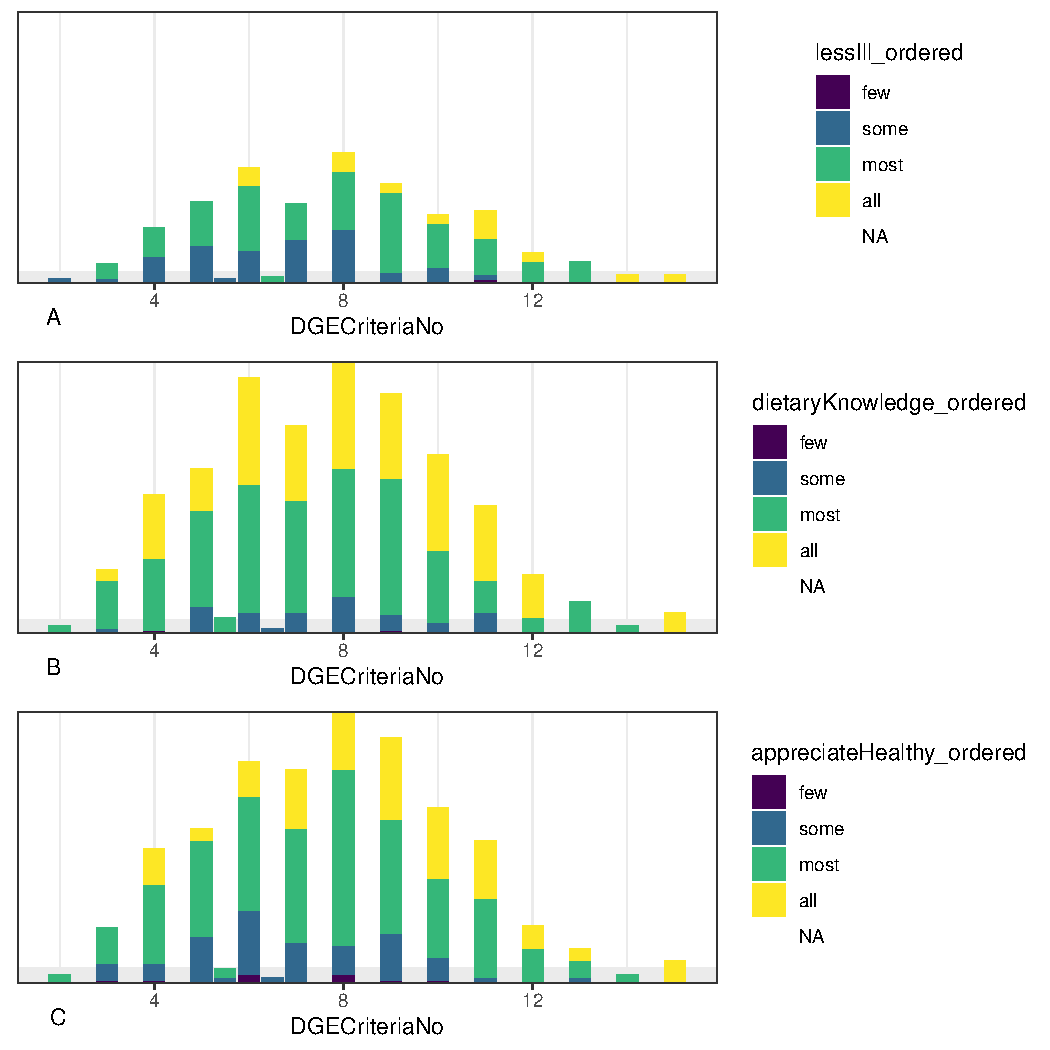
\includegraphics[width=0.8\textwidth]{figure/HealthRegressionsPercentageplots-1} 

}



\end{knitrout}
\floatfoot{DGECriteriaNo is an index that captures how healthy the meals in an organization are. It is based on criteria of the German Nutrition Society (Deutsche Gesellschaft für Ernährung). According to information from CHILDREN, they ask the organizations to send them a sample of their menus. An ecotrophologist collaborating with CHILDREN assessed the menus. In its yearly surveys CHILDREN asks about three variables closley related to a healthy diet. These are the shares of beneficiaries who are healthier (lessIll\_ordered), have a growing appreciation for a healthy diet (dietaryKnowledge\_ordered), or have increased their knowledge about what constitutes a healthy diet (appreciateHealthy\_ordered).
The x-axis plots the index for a healthy diet. The y-axis displays the share of organizarions in each category of the health outcome. The possible values are: all(coded as 4), most (3), some (2), few (1), and none (coded as 0). For example, if an organization says that most beneficiaries are healthier, then this would be coded as 3.}
\end{figure}

In the following equation we use standardized variables in a standard OLS approach. The results are as well compared to the output with the imputed dataset, where we also use scaled coefficents.


\begin{table}
\begin{center}
\scalebox{0.8}{
\begin{tabular}{l c c c c }
\hline
 & OLS & WLS & OLS Impute & WLS Impute \\
\hline
(Intercept)         & $0.02$       & $0.46^{**}$ & $0.09$       & $0.39^{***}$ \\
                    & $(0.08)$     & $(0.16)$    & $(0.07)$     & $(0.12)$     \\
DGECriteriaNoScaled & $0.33^{***}$ & $0.35^{*}$  & $0.25^{***}$ & $0.24$       \\
                    & $(0.08)$     & $(0.16)$    & $(0.07)$     & $(0.14)$     \\
\hline
R$^2$               & 0.12         & 0.29        & 0.07         & 0.16         \\
Adj. R$^2$          & 0.11         & 0.29        & 0.07         & 0.16         \\
Num. obs.           & 121          & 120         & 177          & 177          \\
RMSE                & 0.91         & 7.83        & 0.94         & 7.95         \\
\hline
\multicolumn{5}{l}{\scriptsize{$^{***}p<0.001$, $^{**}p<0.01$, $^*p<0.05$}}
\end{tabular}
}
\caption{Regression Results: Less Ill}
\label{HealthRegressions-LessIll}
\end{center}
\end{table}



\begin{table}
\begin{center}
\scalebox{0.8}{
\begin{tabular}{l c c c c }
\hline
 & OLS & WLS & OLS Impute & WLS Impute \\
\hline
(Intercept)         & $0.02$   & $0.08$   & $0.02$     & $0.21$   \\
                    & $(0.07)$ & $(0.19)$ & $(0.06)$   & $(0.18)$ \\
DGECriteriaNoScaled & $0.11$   & $-0.02$  & $0.12^{*}$ & $0.10$   \\
                    & $(0.06)$ & $(0.12)$ & $(0.05)$   & $(0.14)$ \\
\hline
R$^2$               & 0.01     & 0.00     & 0.02       & 0.01     \\
Adj. R$^2$          & 0.01     & -0.00    & 0.01       & 0.01     \\
Num. obs.           & 214      & 212      & 275        & 275      \\
RMSE                & 0.98     & 8.49     & 0.96       & 9.45     \\
\hline
\multicolumn{5}{l}{\scriptsize{$^{***}p<0.001$, $^{**}p<0.01$, $^*p<0.05$}}
\end{tabular}
}
\caption{Regression Results: Dietary Knowledge}
\label{HealthRegressions-DietaryKnowledge}
\end{center}
\end{table}



\begin{table}
\begin{center}
\scalebox{0.8}{
\begin{tabular}{l c c c c }
\hline
 & OLS & WLS & OLS Impute & WLS Impute \\
\hline
(Intercept)         & $-0.03$      & $0.26$   & $0.02$       & $0.37^{*}$ \\
                    & $(0.07)$     & $(0.18)$ & $(0.06)$     & $(0.17)$   \\
DGECriteriaNoScaled & $0.27^{***}$ & $-0.02$  & $0.25^{***}$ & $0.01$     \\
                    & $(0.07)$     & $(0.15)$ & $(0.06)$     & $(0.13)$   \\
\hline
R$^2$               & 0.06         & 0.00     & 0.06         & 0.00       \\
Adj. R$^2$          & 0.06         & -0.00    & 0.06         & -0.00      \\
Num. obs.           & 213          & 211      & 274          & 274        \\
RMSE                & 1.02         & 8.61     & 1.01         & 9.00       \\
\hline
\multicolumn{5}{l}{\scriptsize{$^{***}p<0.001$, $^{**}p<0.01$, $^*p<0.05$}}
\end{tabular}
}
\caption{Regression Results: Appreciate Healthy}
\label{HealthRegressions-AppreciateHealthy}
\end{center}
\end{table}


\section{Feature Selection}

\subsection{Factor Analysis}

\subsection{Double Selection}

\section{The effect of the "Entdeckerfonds" on the beneficiaries of the program}

How do children benefit from visiting social institutions that CHILDREN supports financially? So far this question could not be empirically validated. Hence, one of the biggest challenges was determining a possible solution for measuring causal effects of the programs on the beneficiaries. During the first meeting with CHILDREN, Wiltrud de Haan presented relevant information that CHILDREN supports all organizations with the Mittagstisch program. However, not all organizations do receive addtitional funding to provide the Entdeckerfonds program. This fact could be used for applying an empirical approach which determines causal effects of the Entdeckerfonds program by comparing a treatment with a control group. The aim of this analysis is to show that the trips provided by Entdeckerfonds program funding have a positive effect on selfworth and everyday expertise of the participating children. 

Empirical Approach\\

The baseline of the empirical approach is the determination of the treatment and control group. Using the data provided by children we specify the treatment group as all organizations that receive funding for both the Entdeckerfonds and the Mittagstisch program. On the other hand, the control group represents all organizations that do not receive funding from CHILDREN to provide the Entdeckerfonds.

Determining the treatment and control group this way, however, was a problem.

THerefore we used the cleaned data set and only determined the control group - all organizations that have no values/answers for the questions of the Entdeckerfonds. We assume that these organizations did not receive the funding for the Entdeckerfonds and therefore are the control group in our analysis. All organizations that gave answers to at least one question of the survey part regarding the entdeckerfonds are considered the treatment group. 
Our analysis is based on this very strong definition of the treatment and control group.

Because we do not have data for the entdeckerfonds survey for the control group as this group is not observed we use the answers of the mittagstisch survey for our analysis. THerefore our possible dependent variables are limited as most of the questions are specific to the meals program. 

As the dataset does not include the variables for the Entdeckerfonds survey for the control group, the potential outcomes regarding the Entdeckerfonds are not observed. Therefore we have to use the survey answers from the Mittagstisch survey.

Generally our data set contains variables from the years 2011 until 2018. 

The constellation of the treatment and control group varies from year to year. 
Assumption: erhalten der treatment gleichbedeutend wie ein verlust

Possible variables as dependent variables
how we determined that:
The used variables should not be specific to the mittagstisch but more general and should also apply to the context of the Entdeckerfonds
possible variables selfworth, day to day skills
used these variables because these variables could be influenced both by the mittagstisch and entdeckerfonds and are not specific to the entdeckerfonds

looked at the general trends of these two variables with the difference of the treatment and control group to look at whether our idea makes sense

linear regression just to look at whether there are effects

add controls and fixed effects time and id fixedeffects --> explain why (id: specific effects of being in Bayern for example or the subsidy amount)
how fixed effects are implemented

which control variables we use
how we determined which controls


\begin{table}
\begin{center}
\begin{tabular}{l c}
\hline
 & Selfworth \\
\hline
(Intercept)             & $-1.13^{***}$ \\
                        & $(0.32)$      \\
dfcEF2$treatEF          & $-0.47$       \\
                        & $(0.31)$      \\
\hline
Num. obs.               & $430$         \\
R$^2$ (full model)      & $0.47$        \\
R$^2$ (proj model)      & $0.47$        \\
Adj. R$^2$ (full model) & $0.36$        \\
Adj. R$^2$ (proj model) & $0.36$        \\
\hline
\multicolumn{2}{l}{\scriptsize{$^{***}p<0.001$; $^{**}p<0.01$; $^{*}p<0.05$}}
\end{tabular}
\caption{linear regression}
\label{table:coefficients}
\end{center}
\end{table}




Ende??
the dataset does not allow a channel analysis but these could be possible channels that might explain the effects we find


% Table created by stargazer v.5.2.2 by Marek Hlavac, Harvard University. E-mail: hlavac at fas.harvard.edu
<<<<<<< HEAD
% Date and time: Mi, Feb 26, 2020 - 23:16:52
=======
% Date and time: Wed, Feb 26, 2020 - 10:15:19 PM
>>>>>>> 72c6d5913679c3fb04935b691d8cdf7883ee60c8
% Requires LaTeX packages: dcolumn rotating 
\begin{sidewaystable}[!htbp] \centering 
  \caption{Regression Results} 
  \label{} 
\begin{tabular}{@{\extracolsep{5pt}}lD{.}{.}{-3} D{.}{.}{-3} D{.}{.}{-3} D{.}{.}{-3} } 
\\[-1.8ex]\hline 
\hline \\[-1.8ex] 
 & \multicolumn{4}{c}{\textit{Dependent variable:}} \\ 
\cline{2-5} 
\\[-1.8ex] & \multicolumn{4}{c}{selfworth} \\ 
\\[-1.8ex] & \multicolumn{1}{c}{(1)} & \multicolumn{1}{c}{(2)} & \multicolumn{1}{c}{(3)} & \multicolumn{1}{c}{(4)}\\ 
\hline \\[-1.8ex] 
 Constant & 2.796^{***} & 2.870^{***} & 2.774^{***} & 2.847^{***} \\ 
  & (0.065) & (0.095) & (0.092) & (0.107) \\ 
  & & & & \\ 
 treatEF & 0.249^{***} & 0.320^{***} & 0.253^{***} & 0.333^{***} \\ 
  & (0.074) & (0.097) & (0.075) & (0.100) \\ 
  & & & & \\ 
\hline \\[-1.8ex] 
ID fixed effects & No & No & Yes & Yes \\ 
Time fixed effects & No & Yes & No & Yes \\ 
Observations & \multicolumn{1}{c}{430} & \multicolumn{1}{c}{430} & \multicolumn{1}{c}{430} & \multicolumn{1}{c}{430} \\ 
R$^{2}$ & \multicolumn{1}{c}{0.026} & \multicolumn{1}{c}{0.035} & \multicolumn{1}{c}{0.026} & \multicolumn{1}{c}{0.036} \\ 
Adjusted R$^{2}$ & \multicolumn{1}{c}{0.024} & \multicolumn{1}{c}{0.017} & \multicolumn{1}{c}{0.022} & \multicolumn{1}{c}{0.015} \\ 
Residual Std. Error & \multicolumn{1}{c}{0.642 (df = 428)} & \multicolumn{1}{c}{0.644 (df = 421)} & \multicolumn{1}{c}{0.642 (df = 427)} & \multicolumn{1}{c}{0.645 (df = 420)} \\ 
F Statistic & \multicolumn{1}{c}{11.417$^{***}$ (df = 1; 428)} & \multicolumn{1}{c}{1.916$^{*}$ (df = 8; 421)} & \multicolumn{1}{c}{5.752$^{***}$ (df = 2; 427)} & \multicolumn{1}{c}{1.724$^{*}$ (df = 9; 420)} \\ 
\hline 
\hline \\[-1.8ex] 
\textit{Note:}  & \multicolumn{4}{r}{$^{*}$p$<$0.1; $^{**}$p$<$0.05; $^{***}$p$<$0.01} \\ 
\end{tabular} 
\end{sidewaystable} 




\section{Conclusion}

\printbibliography

\section{Appendix}

\subsection{A1: Expanded Health Regression}

In addition to table \ref{HealthRegressions-LessIll} table \ref{expandLessIll} presents the results of an OLS approach with scaled outcomes as well as a WLS approach with scaled outcomes with following control variables: to which extent an organization uses regional products, since when an organization is part of the Lunch program, the real subsidy per beneficiary and the state an organization is located. 

% #normal weights selfworth& subsidiy
% <<eqaulity_extra_reg, echo=FALSE, results='asis', message=FALSE, warning=FALSE>>=
% 
% lm_s = readRDS("./ANALYSIS/Tables/selfworth.lm.Rds") #weighted
% lm_d = readRDS("./ANALYSIS/Tables/dayToDaySkills.lm.Rds") #weighted
% ts = readRDS("./ANALYSIS/Tables/selfworthTrips.lm.Rds")
% td = readRDS("./ANALYSIS/Tables/dayToDaySkillsTrips.lm.Rds")
% sI = readRDS("./ANALYSIS/Tables/selfworth_IM.lm.Rds") #weighted
% dI = readRDS("./ANALYSIS/Tables/dayToDaySkills_IM.lm.Rds") #weighted
% tsI = readRDS("./ANALYSIS/Tables/selfworthTrips_IM.lm.Rds")
% tdI = readRDS("./ANALYSIS/Tables/dayToDaySkillsTrips_IM.lm.Rds")
% @


\begin{table}
\begin{center}
\scalebox{0.8}{
\begin{tabular}{l c c c c }
\hline
 & OLS & WLS & OLS Impute & WLS Impute \\
\hline
(Intercept)               & $-1.08^{***}$ & $-0.99^{**}$ & $0.02$      & $-0.08$    \\
                          & $(0.24)$      & $(0.30)$     & $(0.15)$    & $(0.20)$   \\
DGECriteriaNoScaled       & $0.34^{***}$  & $0.36^{***}$ & $0.19^{**}$ & $0.27$     \\
                          & $(0.08)$      & $(0.06)$     & $(0.07)$    & $(0.14)$   \\
regionalProducts\_scaled  & $0.02$        & $-0.03$      & $0.11$      & $0.02$     \\
                          & $(0.08)$      & $(0.11)$     & $(0.07)$    & $(0.11)$   \\
yearsSupportSince         & $0.02$        & $-0.03$      & $-0.01$     & $0.05^{*}$ \\
                          & $(0.03)$      & $(0.04)$     & $(0.02)$    & $(0.02)$   \\
realSubsidyPerBeneficiary & $-0.00$       & $0.00$       &             & $-0.00$    \\
                          & $(0.00)$      & $(0.00)$     &             & $(0.00)$   \\
stateBayern               & $0.96^{**}$   & $1.88^{***}$ &             &            \\
                          & $(0.33)$      & $(0.49)$     &             &            \\
stateBerlin               & $1.09^{**}$   & $1.34^{***}$ &             &            \\
                          & $(0.37)$      & $(0.37)$     &             &            \\
stateBrandenburg          & $2.21^{***}$  & $2.46^{***}$ &             &            \\
                          & $(0.43)$      & $(0.40)$     &             &            \\
stateBremen               & $1.00$        & $1.03$       &             &            \\
                          & $(0.58)$      & $(0.59)$     &             &            \\
stateHamburg              & $0.95$        & $1.96^{***}$ &             &            \\
                          & $(0.67)$      & $(0.40)$     &             &            \\
stateHessen               & $0.87^{***}$  & $1.16^{***}$ &             &            \\
                          & $(0.23)$      & $(0.31)$     &             &            \\
stateMV                   & $0.09$        & $0.14$       &             &            \\
                          & $(0.21)$      & $(0.26)$     &             &            \\
stateNiedersachsen        & $2.48^{***}$  & $2.30^{***}$ &             &            \\
                          & $(0.40)$      & $(0.43)$     &             &            \\
stateNRW                  & $0.68^{*}$    & $1.00^{**}$  &             &            \\
                          & $(0.27)$      & $(0.33)$     &             &            \\
stateSaarland             & $1.50^{***}$  & $1.75^{***}$ &             &            \\
                          & $(0.32)$      & $(0.25)$     &             &            \\
stateSachsen              & $1.34^{***}$  & $1.23^{***}$ &             &            \\
                          & $(0.27)$      & $(0.27)$     &             &            \\
stateSchleswig-Holstein   & $1.33^{***}$  & $1.63^{***}$ &             &            \\
                          & $(0.37)$      & $(0.42)$     &             &            \\
stateThüringen            & $0.99$        & $1.29^{*}$   &             &            \\
                          & $(0.59)$      & $(0.55)$     &             &            \\
realSubsidy               &               &              & $0.00^{**}$ &            \\
                          &               &              & $(0.00)$    &            \\
\hline
R$^2$                     & 0.51          & 0.73         & 0.12        & 0.22       \\
Adj. R$^2$                & 0.39          & 0.66         & 0.10        & 0.20       \\
Num. obs.                 & 88            & 88           & 175         & 175        \\
RMSE                      & 0.73          & 5.62         & 0.92        & 7.77       \\
\hline
\multicolumn{5}{l}{\scriptsize{$^{***}p<0.001$, $^{**}p<0.01$, $^*p<0.05$}}
\end{tabular}
}
\caption{Regression Results: Less ill expanded model}
\label{expandLessIll}
\end{center}
\end{table}


\subsection{A2: Cumulative Odds Regression} 

As an option to run a regression on the original ordinal variables, we use the proportional odds version of the cumulative logit from the VGAM package. Equation \ref{PropoddsModel} describes the model setup: 

 
\begin{equation}
\label{PropoddsModel}
  P(Y_i \leq \ r) = \frac{exp(y_0_r + x_i^Ty)}{1+exp(y_0_r + x_i^Ty)}    
\end{equation}


To demonstrate the results of this method, we show in the tables \ref{lessIllOdds}, \ref{dietaryOdds}, \ref{appreciateOdds} the regressions of the health related variables on the healthy meals criterion and in \ref{selfworthOdds} and \ref{dayToDayOdds} the regressions of the real meals subsidy on selfworth and everyday expertise. 

As an example of interpreting such models, we consider the model of table \ref{lessIllOdds}: An increase of the healthy meals criterion by 1 is associated with an increase in chances, that a proportion of a maximum of r beneficiaries is healthier in relation to that a proportion of more than r beneficiaries are healthier, by the factor of exp(-0.29127) = 0.75.

A summary of the remaining models:

\begin{itemize}
  \item{Dietary Knowledge: exp(-0.089) = 0.91}
  \item{Appreciate Healthy: exp(-0199) = 0.82}
  \item{Selfworth: exp(-0.00001) = 1}
  \item{Everyday Expertise: (-0.00003) = 1} 
\end{itemize}


% Table created by stargazer v.5.2.2 by Marek Hlavac, Harvard University. E-mail: hlavac at fas.harvard.edu
<<<<<<< HEAD
% Date and time: Mi, Feb 26, 2020 - 23:16:52
=======
% Date and time: Wed, Feb 26, 2020 - 10:15:19 PM
>>>>>>> 72c6d5913679c3fb04935b691d8cdf7883ee60c8
% Requires LaTeX packages: dcolumn 
\begin{table}[!htbp] \centering 
  \caption{Propodss Regression Results: Less Ill} 
  \label{lessIllOdds} 
\begin{tabular}{@{\extracolsep{5pt}} D{.}{.}{-3} D{.}{.}{-3} D{.}{.}{-3} D{.}{.}{-3} D{.}{.}{-3} } 
\\[-1.8ex]\hline 
\hline \\[-1.8ex] 
\multicolumn{1}{c}{} & \multicolumn{1}{c}{Estimate} & \multicolumn{1}{c}{Std. Error} & \multicolumn{1}{c}{z value} & \multicolumn{1}{c}{Pr(\textgreater \textbar z\textbar )} \\ 
\hline \\[-1.8ex] 
\multicolumn{1}{c}{(Intercept):1} & -2.799 & 1.109 & -2.523 & 0.012 \\ 
\multicolumn{1}{c}{(Intercept):2} & 1.653 & 0.582 & 2.841 & 0.004 \\ 
\multicolumn{1}{c}{(Intercept):3} & 4.667 & 0.738 & 6.322 & 0 \\ 
\multicolumn{1}{c}{DGECriteriaNo} & -0.291 & 0.075 & -3.883 & 0.0001 \\ 
\hline \\[-1.8ex] 
\end{tabular} 
\end{table} 


% Table created by stargazer v.5.2.2 by Marek Hlavac, Harvard University. E-mail: hlavac at fas.harvard.edu
<<<<<<< HEAD
% Date and time: Mi, Feb 26, 2020 - 23:16:53
=======
% Date and time: Wed, Feb 26, 2020 - 10:15:19 PM
>>>>>>> 72c6d5913679c3fb04935b691d8cdf7883ee60c8
% Requires LaTeX packages: dcolumn 
\begin{table}[!htbp] \centering 
  \caption{Propodss Regression Results: Dietary Knowledge} 
  \label{dietaryOdds} 
\begin{tabular}{@{\extracolsep{5pt}} D{.}{.}{-3} D{.}{.}{-3} D{.}{.}{-3} D{.}{.}{-3} D{.}{.}{-3} } 
\\[-1.8ex]\hline 
\hline \\[-1.8ex] 
\multicolumn{1}{c}{} & \multicolumn{1}{c}{Estimate} & \multicolumn{1}{c}{Std. Error} & \multicolumn{1}{c}{z value} & \multicolumn{1}{c}{Pr(\textgreater \textbar z\textbar )} \\ 
\hline \\[-1.8ex] 
\multicolumn{1}{c}{(Intercept):1} & -4.009 & 0.803 & -4.996 & 0.00000 \\ 
\multicolumn{1}{c}{(Intercept):2} & -1.047 & 0.425 & -2.465 & 0.014 \\ 
\multicolumn{1}{c}{(Intercept):3} & 1.445 & 0.430 & 3.365 & 0.001 \\ 
\multicolumn{1}{c}{DGECriteriaNo} & -0.089 & 0.052 & -1.712 & 0.087 \\ 
\hline \\[-1.8ex] 
\end{tabular} 
\end{table} 


% Table created by stargazer v.5.2.2 by Marek Hlavac, Harvard University. E-mail: hlavac at fas.harvard.edu
<<<<<<< HEAD
% Date and time: Mi, Feb 26, 2020 - 23:16:53
=======
% Date and time: Wed, Feb 26, 2020 - 10:15:19 PM
>>>>>>> 72c6d5913679c3fb04935b691d8cdf7883ee60c8
% Requires LaTeX packages: dcolumn 
\begin{table}[!htbp] \centering 
  \caption{Propodss Regression Results: Appreciate Healthy} 
  \label{appreciateOdds} 
\begin{tabular}{@{\extracolsep{5pt}} D{.}{.}{-3} D{.}{.}{-3} D{.}{.}{-3} D{.}{.}{-3} D{.}{.}{-3} } 
\\[-1.8ex]\hline 
\hline \\[-1.8ex] 
\multicolumn{1}{c}{} & \multicolumn{1}{c}{Estimate} & \multicolumn{1}{c}{Std. Error} & \multicolumn{1}{c}{z value} & \multicolumn{1}{c}{Pr(\textgreater \textbar z\textbar )} \\ 
\hline \\[-1.8ex] 
\multicolumn{1}{c}{(Intercept):1} & -1.603 & 0.486 & -3.298 & 0.001 \\ 
\multicolumn{1}{c}{(Intercept):2} & 0.586 & 0.413 & 1.419 & 0.156 \\ 
\multicolumn{1}{c}{(Intercept):3} & 3.052 & 0.471 & 6.483 & 0 \\ 
\multicolumn{1}{c}{DGECriteriaNo} & -0.199 & 0.053 & -3.744 & 0.0002 \\ 
\hline \\[-1.8ex] 
\end{tabular} 
\end{table} 



% Table created by stargazer v.5.2.2 by Marek Hlavac, Harvard University. E-mail: hlavac at fas.harvard.edu
<<<<<<< HEAD
% Date and time: Mi, Feb 26, 2020 - 23:16:53
=======
% Date and time: Wed, Feb 26, 2020 - 10:15:19 PM
>>>>>>> 72c6d5913679c3fb04935b691d8cdf7883ee60c8
% Requires LaTeX packages: dcolumn 
\begin{table}[!htbp] \centering 
  \caption{Propodss Regression Results: Selfworth} 
  \label{selfworthOdds} 
\begin{tabular}{@{\extracolsep{5pt}} D{.}{.}{-3} D{.}{.}{-3} D{.}{.}{-3} D{.}{.}{-3} D{.}{.}{-3} } 
\\[-1.8ex]\hline 
\hline \\[-1.8ex] 
\multicolumn{1}{c}{} & \multicolumn{1}{c}{Estimate} & \multicolumn{1}{c}{Std. Error} & \multicolumn{1}{c}{z value} & \multicolumn{1}{c}{Pr(\textgreater \textbar z\textbar )} \\ 
\hline \\[-1.8ex] 
\multicolumn{1}{c}{(Intercept):1} & -4.855 & 0.584 & -8.315 & 0 \\ 
\multicolumn{1}{c}{(Intercept):2} & -1.268 & 0.143 & -8.893 & 0 \\ 
\multicolumn{1}{c}{(Intercept):3} & 1.514 & 0.150 & 10.109 & 0 \\ 
\multicolumn{1}{c}{realSubsidy} & -0.00001 & 0.00001 & -1.332 & 0.183 \\ 
\hline \\[-1.8ex] 
\end{tabular} 
\end{table} 



% Table created by stargazer v.5.2.2 by Marek Hlavac, Harvard University. E-mail: hlavac at fas.harvard.edu
<<<<<<< HEAD
% Date and time: Mi, Feb 26, 2020 - 23:16:53
=======
% Date and time: Wed, Feb 26, 2020 - 10:15:19 PM
>>>>>>> 72c6d5913679c3fb04935b691d8cdf7883ee60c8
% Requires LaTeX packages: dcolumn 
\begin{table}[!htbp] \centering 
  \caption{Propodss Regression Results: Everyday expertise} 
  \label{dayToDayOdds} 
\begin{tabular}{@{\extracolsep{5pt}} D{.}{.}{-3} D{.}{.}{-3} D{.}{.}{-3} D{.}{.}{-3} D{.}{.}{-3} } 
\\[-1.8ex]\hline 
\hline \\[-1.8ex] 
\multicolumn{1}{c}{} & \multicolumn{1}{c}{Estimate} & \multicolumn{1}{c}{Std. Error} & \multicolumn{1}{c}{z value} & \multicolumn{1}{c}{Pr(\textgreater \textbar z\textbar )} \\ 
\hline \\[-1.8ex] 
\multicolumn{1}{c}{(Intercept):1} & -3.543 & 0.343 & -10.330 & 0 \\ 
\multicolumn{1}{c}{(Intercept):2} & -0.736 & 0.132 & -5.563 & 0.00000 \\ 
\multicolumn{1}{c}{(Intercept):3} & 1.764 & 0.157 & 11.249 & 0 \\ 
\multicolumn{1}{c}{realSubsidy} & -0.00003 & 0.00001 & -4.070 & 0.00005 \\ 
\hline \\[-1.8ex] 
\end{tabular} 
\end{table} 


\subsection{A3: Partition}

In addition to the factor analysis described in section 6, we would like to introduce to a another dimensionality reduction method called partition. 

QUOTES FROM PAPER, describe method 

In the following a threshold of 0.4 is used, meaning that the reduced variable consists of variables which explain each other to at least 40 percent. It might be meaningful to decide to use only one of the variables a reduced variable consists of or a summarizing one for future surveys to avoid redundancy. Table x shows the obtained results of the dimensionality reduction and displays x variables which haven't been reduced, and x reduced ones.    

% latex table generated in R 3.6.2 by xtable 1.8-4 package
<<<<<<< HEAD
% Wed Feb 26 23:16:53 2020
=======
% Wed Feb 26 22:15:20 2020
>>>>>>> 72c6d5913679c3fb04935b691d8cdf7883ee60c8
\begin{table}[ht]
\centering
\begin{tabular}{rllr}
  \hline
 & Variable, Meals & Mapping, Meals & Information, Meals \\ 
  \hline
1 & participateMore & participateMore & 1.00 \\ 
  2 & tasksLunch & tasksLunch & 1.00 \\ 
  3 & ownIdeas & ownIdeas & 1.00 \\ 
  4 & stayLonger & stayLonger & 1.00 \\ 
  5 & dietaryKnowledge & dietaryKnowledge & 1.00 \\ 
  6 & appreciateHealthy & appreciateHealthy & 1.00 \\ 
  7 & foodCulture & foodCulture & 1.00 \\ 
  8 & lessIll & lessIll & 1.00 \\ 
  9 & betterTeamwork & betterTeamwork & 1.00 \\ 
  10 & moreRegularSchoolVisits & moreRegularSchoolVisits & 1.00 \\ 
  11 & addressProblems & addressProblems & 1.00 \\ 
  12 & reduced\_var\_1 & moreConcentrated & 0.66 \\ 
  13 & reduced\_var\_1 & moreBalanced & 0.66 \\ 
  14 & reduced\_var\_2 & monthlyCooks & 0.42 \\ 
  15 & reduced\_var\_2 & weeklyCooks & 0.42 \\ 
  16 & reduced\_var\_2 & shoppers & 0.42 \\ 
  17 & reduced\_var\_2 & easyDishes & 0.42 \\ 
  18 & reduced\_var\_3 & dayToDaySkills & 0.43 \\ 
  19 & reduced\_var\_3 & moreIndependent & 0.43 \\ 
  20 & reduced\_var\_3 & selfworth & 0.43 \\ 
  21 & reduced\_var\_3 & moreOpen & 0.43 \\ 
  22 & reduced\_var\_3 & moreConfidence & 0.43 \\ 
  23 & reduced\_var\_3 & proud & 0.43 \\ 
  24 & reduced\_var\_4 & betterReading & 0.53 \\ 
  25 & reduced\_var\_4 & betterNumbers & 0.53 \\ 
  26 & reduced\_var\_4 & betterGrades & 0.53 \\ 
  27 & reduced\_var\_5 & influenceHome & 0.41 \\ 
  28 & reduced\_var\_5 & cookAtHome & 0.41 \\ 
  29 & reduced\_var\_5 & askRecipes & 0.41 \\ 
   \hline
\end{tabular}
\caption{Partition of outcomes, Meals} 
\end{table}
% latex table generated in R 3.6.2 by xtable 1.8-4 package
<<<<<<< HEAD
% Wed Feb 26 23:16:53 2020
=======
% Wed Feb 26 22:15:20 2020
>>>>>>> 72c6d5913679c3fb04935b691d8cdf7883ee60c8
\begin{table}[ht]
\centering
\begin{tabular}{rllr}
  \hline
 & Variable, Trips & Mapping, Trips & Information, Trips \\ 
  \hline
1 & tripsSuggestions & tripsSuggestions & 1.00 \\ 
  2 & tripsDecisions & tripsDecisions & 1.00 \\ 
  3 & tripsOrganization & tripsOrganization & 1.00 \\ 
  4 & tripsCostCalculation & tripsCostCalculation & 1.00 \\ 
  5 & tripsBudget & tripsBudget & 1.00 \\ 
  6 & tripsMoney & tripsMoney & 1.00 \\ 
  7 & tripsReview & tripsReview & 1.00 \\ 
  8 & tripsPublicTransport & tripsPublicTransport & 1.00 \\ 
  9 & tripsMobility & tripsMobility & 1.00 \\ 
  10 & tripsAdditionalActivities & tripsAdditionalActivities & 1.00 \\ 
  11 & tripsSelfworth & tripsSelfworth & 1.00 \\ 
  12 & tripsFrustrationTolerance & tripsFrustrationTolerance & 1.00 \\ 
  13 & reduced\_var\_1 & tripsSuccess & 0.68 \\ 
  14 & reduced\_var\_1 & tripsSelfEfficacy & 0.68 \\ 
  15 & reduced\_var\_2 & tripsNewPlaces & 0.60 \\ 
  16 & reduced\_var\_2 & tripsNewCommunities & 0.60 \\ 
  17 & reduced\_var\_2 & tripsNewIdeas & 0.60 \\ 
  18 & reduced\_var\_2 & tripsSocialSkills & 0.60 \\ 
  19 & reduced\_var\_3 & tripsSpecificSkills & 0.46 \\ 
  20 & reduced\_var\_3 & tripsDayToDaySkills & 0.46 \\ 
   \hline
\end{tabular}
\caption{Partition of outcomes, Trips} 
\end{table}
\begin{kframe}

<<<<<<< HEAD
{\ttfamily\noindent\bfseries\color{errorcolor}{\#\# Error in print.default(m, ..., quote = quote, right = right, max = max): ungültiges 'digits' Argument}}\end{kframe}
=======
{\ttfamily\noindent\bfseries\color{errorcolor}{\#\# Error in print.default(m, ..., quote = quote, right = right, max = max): invalid 'digits' argument}}\end{kframe}
\subsection{A3: OLS Regressions}

#normal weights selfworth& subsidiy


% <<lessIll_extra_reg, echo=FALSE, results='asis', message=FALSE, warning=FALSE>>=
% #expanded model less ill 
% 
% lm_elDGE = readRDS("./ANALYSIS/Tables/Expand_LessIll_scaled.Rds")
% lm_elDGEw = readRDS("./ANALYSIS/Tables/Expand_LessIll_scaled_weighted.Rds")
% elDGE_iw = readRDS("./ANALYSIS/Tables/Expand_LessIll_IM_scaled_weighted.Rds")
% @
>>>>>>> 72c6d5913679c3fb04935b691d8cdf7883ee60c8

\section{Ehrenwörtliche Erklärung aller Teilnehmer}


\end{document}
